\documentclass{summarysheet}

\begin{document}


\maketitle{5}{Potential Energy and the Electric Potential}

\begin{multicols}{2}

\begin{topicbox}{Mechanical Energy Conservation}

\noindent Recall that in isolated, dissipationless systems. the mechanical energy is conserved:
\[
K_i + U_i = K_f + U_f.
\]
The potential energy depends on the type of interaction between objects.
\end{topicbox}

\begin{topicbox}{Electric Potential Energy}

\noindent If two point charges a distance $r$ apart interact through the electric force, they have a potential energy given by
\begin{teqbox}
\[
U_\text{elec} = \frac{1}{4\pi \epsilon_0} \frac{q_1 q_2}{r}.
\]
\end{teqbox}
\noindent With three or more point charges interacting, the electric potential energy must be calculated by summing over all pairs $(i, j)$ of particles:
\begin{teqbox}
\[
U_\text{elec} = \sum_{i<j} \frac{1}{4\pi \epsilon_0} \frac{q_i q_j}{r_{ij}}.
\]
\end{teqbox}

\begin{multicols}{2}
\noindent When an electric dipole interacts with a constant electric field $\vec{E}$, the potential energy of the system is
\[
U_\text{elec} = -\vec{p} \cdot \vec{E},
\]
\begin{center}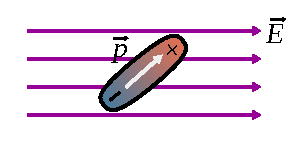
\includegraphics[scale=0.6]{fig_dipole.pdf}\end{center}
\end{multicols}
\noindent where $\vec{p}$ is the dipole moment with magnitude $p = qs$.


\end{topicbox}


\begin{topicbox}{Electric Field and Potential}
\begin{multicols}{2}
\noindent The electric field and the electric potential are related in the same way that force and potential energy are related.  Mathematically,
\[
\Delta V = V_f - V_i = - \int_{s_i}^{s_f} E_s \, ds
\]
and
\[
E_s = -\frac{dV}{ds}.
\]
\begin{center}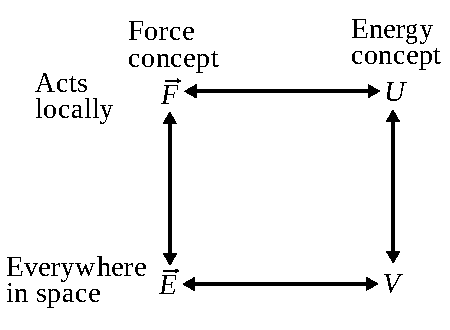
\includegraphics[scale=0.6]{fig_field_pot.pdf}\end{center}
\end{multicols}

\begin{multicols}{2}
\noindent Graphically, we can see the relationship with field lines and equipotential surfaces:
\begin{itemize}
\item $\vec{E}$ is perpendicular to the equipotential surfaces.
\item $\vec{E}$ points from higher to lower potential.
\item $\vec{E}$ is greater in magnitude where the equipotential surfaces are closer together.
\end{itemize}
\begin{center}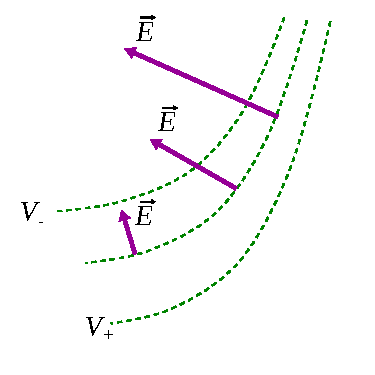
\includegraphics[scale=0.6]{fig_equi_lines.pdf}\end{center}
\end{multicols}

\vspace{0.35in}

\end{topicbox}



\end{multicols}

\begin{topicbox}{Electric Potential}
\begin{multicols}{2}
The electric potential is another way to describe the alteration of space created by charge. It is defined through its effect on a test charge $q$:
\begin{teqbox}
\[
V = \frac{U_\text{$q + $ sources}}{q}.
\]
\end{teqbox}
\noindent From this definition, we see that a point charge $q$ in an electric potential $V$ has potential energy 
\begin{teqbox}
\[
U_\text{elec} = qV.
\]
\end{teqbox}
\noindent The unit of the electric potential is the \emph{volt}, 1 V = 1 J/C.

\vspace{0.1in}

\begin{multicols}{2}
\noindent \textbf{Potential inside a capacitor}: 

\begin{eqbox}
V = Es
\end{eqbox}
\begin{center}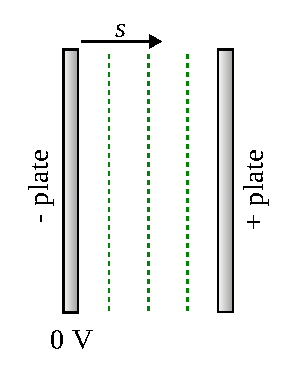
\includegraphics[scale=0.55]{fig_cap.pdf}\end{center}


\noindent \textbf{Potential of a point charge}:
\begin{eqbox}
V = \frac{1}{4\pi \epsilon_0} \frac{q}{r}
\end{eqbox}
\begin{center}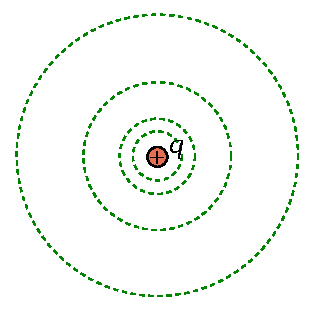
\includegraphics[scale=0.6]{fig_pt_charge.pdf}\end{center}
\end{multicols}


\noindent \textbf{Potential of multiple point charges}:
\begin{multicols}{2}
\begin{eqbox}
V = \sum_i\frac{1}{4\pi \epsilon_0} \frac{q_i}{r_i}
\end{eqbox}
\begin{center}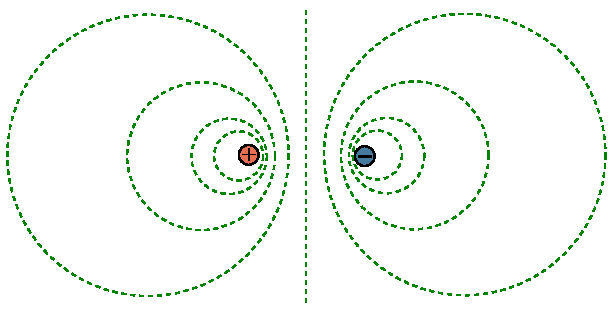
\includegraphics[scale=0.4]{fig_pt_charges.pdf}\end{center}
\end{multicols}

\noindent \textbf{Potential of continuous charge distributions}

\begin{multicols}{2}

\noindent If the charge distribution is continuous, we again use the \emph{principle of superposition:}
\begin{enumerate}
\item Divide the total charge $Q$ of the object into many small charges $dQ$, each of which acts like a point charge.
\item Find the electric potential $dV$ of each small charge $dQ$.
\item Add all electric potential $dV$ together by integrating over the object to find the net potential $V$.
\end{enumerate}
But remember: the electric potential is a \emph{scalar}, so you don’t need to break it up into $x$ and $y$ components.
\begin{center}
\includegraphics[scale=0.7]{fig_continuous.pdf}\end{center}

\end{multicols}


\end{multicols}




\end{topicbox}






\makebanner{Electricity and Magnetism}

\end{document}



